\documentclass[conference]{IEEEtran}
\IEEEoverridecommandlockouts

\usepackage{cite}
\usepackage{amsmath,amssymb,amsfonts}
\usepackage{graphicx}
\usepackage{textcomp}
\usepackage{xcolor}
\usepackage{array}
\usepackage{url}
\usepackage{tikz}
\usetikzlibrary{arrows.meta,positioning}

\def\BibTeX{{\rm B\kern-.05em{\sc i\kern-.025em b}\kern-.08em
		T\kern-.1667em\lower.7ex\hbox{E}\kern-.125emX}}
\begin{document}
	
	\title{Original Method: Data-Driven Approximation of Earth--Mars Pork-Chop Surfaces}
	
	\author{\IEEEauthorblockN{Scott Nguyen}
		\IEEEauthorblockA{\textit{Dept. of Electrical and Computer Engineering} \\
			\textit{University of New Mexico}\\
			Albuquerque, NM, USA \\
			scott.nguyen@example.edu}
	}
	
	\maketitle
	
	\begin{abstract}
		This proposal presents an original method that integrates data-driven modeling with classical interplanetary trajectory analysis. A surrogate model will be trained on synthetically generated Earth--Mars transfer data to approximate optimal $\Delta V$ and time-of-flight (TOF) values. The goal is to reproduce the characteristic \emph{pork-chop surface}---the map of launch windows, $\Delta V$, and TOF---while significantly reducing computational effort compared to traditional solvers. This aligns with recent efforts to replace traditional solvers with neural-network surrogates for trajectory optimization and robust design under uncertainty~\cite{ruff2023surrogate,federici2024robust,zavoli2021reinforcement}.
	\end{abstract}
	
	\begin{IEEEkeywords}
		pork-chop plot, trajectory optimization, Earth--Mars transfer, surrogate modeling, interplanetary dynamics
	\end{IEEEkeywords}
	
	\section{Motivation}
	Designing interplanetary trajectories involves solving complex nonlinear equations to determine feasible transfers between planets. Traditional tools such as Lambert solvers require repeated iterations to search launch windows, increasing computational load~\cite{zavoli2021reinforcement}. The resulting trade space between departure date, arrival date, $\Delta V$, and TOF is visualized using a \emph{pork-chop plot}, which is still a standard tool in preliminary interplanetary mission design.
	
	Recent literature shows success using neural networks and reinforcement learning to approximate or optimize trajectory costs without repeatedly solving differential equations. Ruff \textit{et al.} demonstrate how surrogate neural networks can approximate simulation-based trajectory optimization~\cite{ruff2023surrogate}, while Federici \textit{et al.} and Zavoli \textit{et al.} apply meta-reinforcement learning to robust trajectory design under multiple uncertainties~\cite{federici2024robust,zavoli2021reinforcement}. These works motivate the current project to explore an Earth--Mars surrogate model targeting rapid pork-chop surface recreation.
	
	\section{Expected Contribution}
	This project will produce a reproducible workflow that:
	\begin{itemize}
		\item Generates a synthetic Earth--Mars transfer dataset using numerical trajectory solutions based on Lambert’s problem~\cite{ruff2023surrogate}.
		\item Trains a surrogate model to approximate $\Delta V$ and TOF from input geometry and timing data.
		\item Documents training and validation using Google Colab tutorials with full reproducibility and clear structure.
		\item Evaluates model performance using visual and quantitative metrics, aligned with standards in surrogate-based trajectory design research~\cite{ruff2023surrogate,federici2024robust}.
	\end{itemize}
	
	\section{Expected Contribution Against Competitive Methods}
	\begin{table}[h]
		\caption{Comparison with Existing Methods}
		\centering
		\resizebox{\columnwidth}{!}{
			\begin{tabular}{|p{2.1cm}|p{2.0cm}|p{1.9cm}|p{2.2cm}|}
				\hline
				\textbf{Method} & \textbf{Key Feature} & \textbf{Limitation} & \textbf{New Element in This Project} \\ \hline
				Classical Lambert Solver & Analytic, deterministic & Requires iteration per case & Learns entire $\Delta V$ surface \\ \hline
				Direct Optimization & Accurate baseline & Slow over large launch windows & Provides labeled reference data for training \\ \hline
				Surrogate NN~\cite{ruff2023surrogate} & Fast cost predictions & Requires dataset setup & Predicts pork-chop trade space directly \\ \hline
				Meta-RL~\cite{zavoli2021reinforcement,federici2024robust} & Handles uncertainties via learned policies & Complex training and deployment & Surrogate trades some accuracy for speed and simplicity \\ \hline
			\end{tabular}
		}
		\label{tab:comparison}
	\end{table}
	
	\section{Draft Flowchart / Pseudocode}
	\textbf{Workflow Overview:}
	\begin{enumerate}
		\item Generate Earth--Mars transfer samples using a Lambert solver.
		\item Record corresponding $\Delta V$ and TOF for each valid trajectory.
		\item Store data in structured files and split into training, validation, and testing sets.
		\item Train a surrogate model using appropriate optimization and validation steps.
		\item Evaluate prediction accuracy and timing efficiency.
		\item Test on launch opportunities beyond the training window.
	\end{enumerate}
	
	To make the workflow clearer and to satisfy the project requirement for a flowchart, Fig.~\ref{fig:flowchart} summarizes the proposed pipeline from data generation to surrogate evaluation.
	
\begin{figure}[h]
	\centering
	\scriptsize
	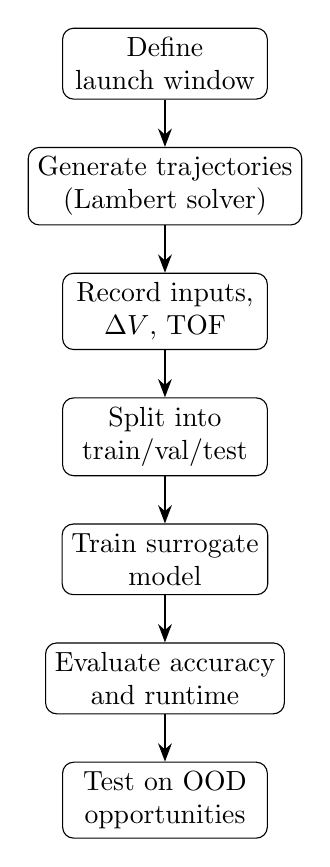
\begin{tikzpicture}[
		node distance=0.6cm,
		block/.style={
			rectangle,
			draw,
			rounded corners,
			align=center,
			minimum width=2.6cm,
			minimum height=0.7cm
		},
		arrow/.style={-{Stealth}, thick}
		]
		\node[block] (start) {Define\\launch window};
		\node[block, below=of start] (lambert) {Generate trajectories\\(Lambert solver)};
		\node[block, below=of lambert] (record) {Record inputs,\\$\Delta V$, TOF};
		\node[block, below=of record] (split) {Split into\\train/val/test};
		\node[block, below=of split] (train) {Train surrogate\\model};
		\node[block, below=of train] (eval) {Evaluate accuracy\\and runtime};
		\node[block, below=of eval] (ood) {Test on OOD\\opportunities};
		
		\draw[arrow] (start) -- (lambert);
		\draw[arrow] (lambert) -- (record);
		\draw[arrow] (record) -- (split);
		\draw[arrow] (split) -- (train);
		\draw[arrow] (train) -- (eval);
		\draw[arrow] (eval) -- (ood);
	\end{tikzpicture}
	\caption{Flowchart of the proposed Earth--Mars pork-chop surrogate workflow.}
	\label{fig:flowchart}
\end{figure}

	\section{Code Implementation}
	The project will be implemented in \textbf{Google Colab}, following the required tutorial format. Each tutorial will include:
	\begin{itemize}
		\item Documentation using markdown text and headings.
		\item Installation and version notes for all required packages.
		\item Clear explanations of dataset setup, model training, and testing steps.
		\item Approximate runtime information and hardware specifications.
	\end{itemize}
	This organization mirrors reproducible practices in recent surrogate model development for trajectory planning~\cite{ruff2023surrogate}.
	
	\section{Dataset Requirements}
	\subsection{Source and Description}
	A synthetic dataset will be generated by solving Earth--Mars transfer cases across multiple synodic periods using a two-body approximation, consistent with prior surrogate modeling work~\cite{ruff2023surrogate}.
	\begin{itemize}
		\item \textbf{Inputs:} departure epoch, arrival epoch, planetary longitudes, and synodic phase angle.
		\item \textbf{Outputs:} total $\Delta V$ [km/s], TOF [days].
		\item \textbf{Size:} approximately 1000 samples.
		\item \textbf{Format:} stored as \texttt{.csv} files in \texttt{training}, \texttt{validation}, and \texttt{testing} subdirectories.
	\end{itemize}
	
	\subsection{Splitting and Independence}
	Data will be split 70\% for training, 15\% for validation, and 15\% for testing. An additional out-of-distribution (OOD) set from a distinct synodic period will test generalization, similar to robustness checks in meta-RL trajectory work~\cite{federici2024robust}.
	
	\subsection{Data Documentation Figure}
	Figure~\ref{fig:dataset} presents a synthetic Earth--Mars \textbf{pork-chop plot}, which visualizes contours of total $\Delta V$ as a function of departure epoch and time-of-flight. The repeating low-$\Delta V$ windows correspond to Hohmann-like transfer opportunities occurring roughly every 26 months. The surrogate model aims to reproduce these low-cost corridors in a data-driven fashion, inspired by the surrogate mapping of cost landscapes in~\cite{ruff2023surrogate}.
	\begin{figure}[h]
		\centering
		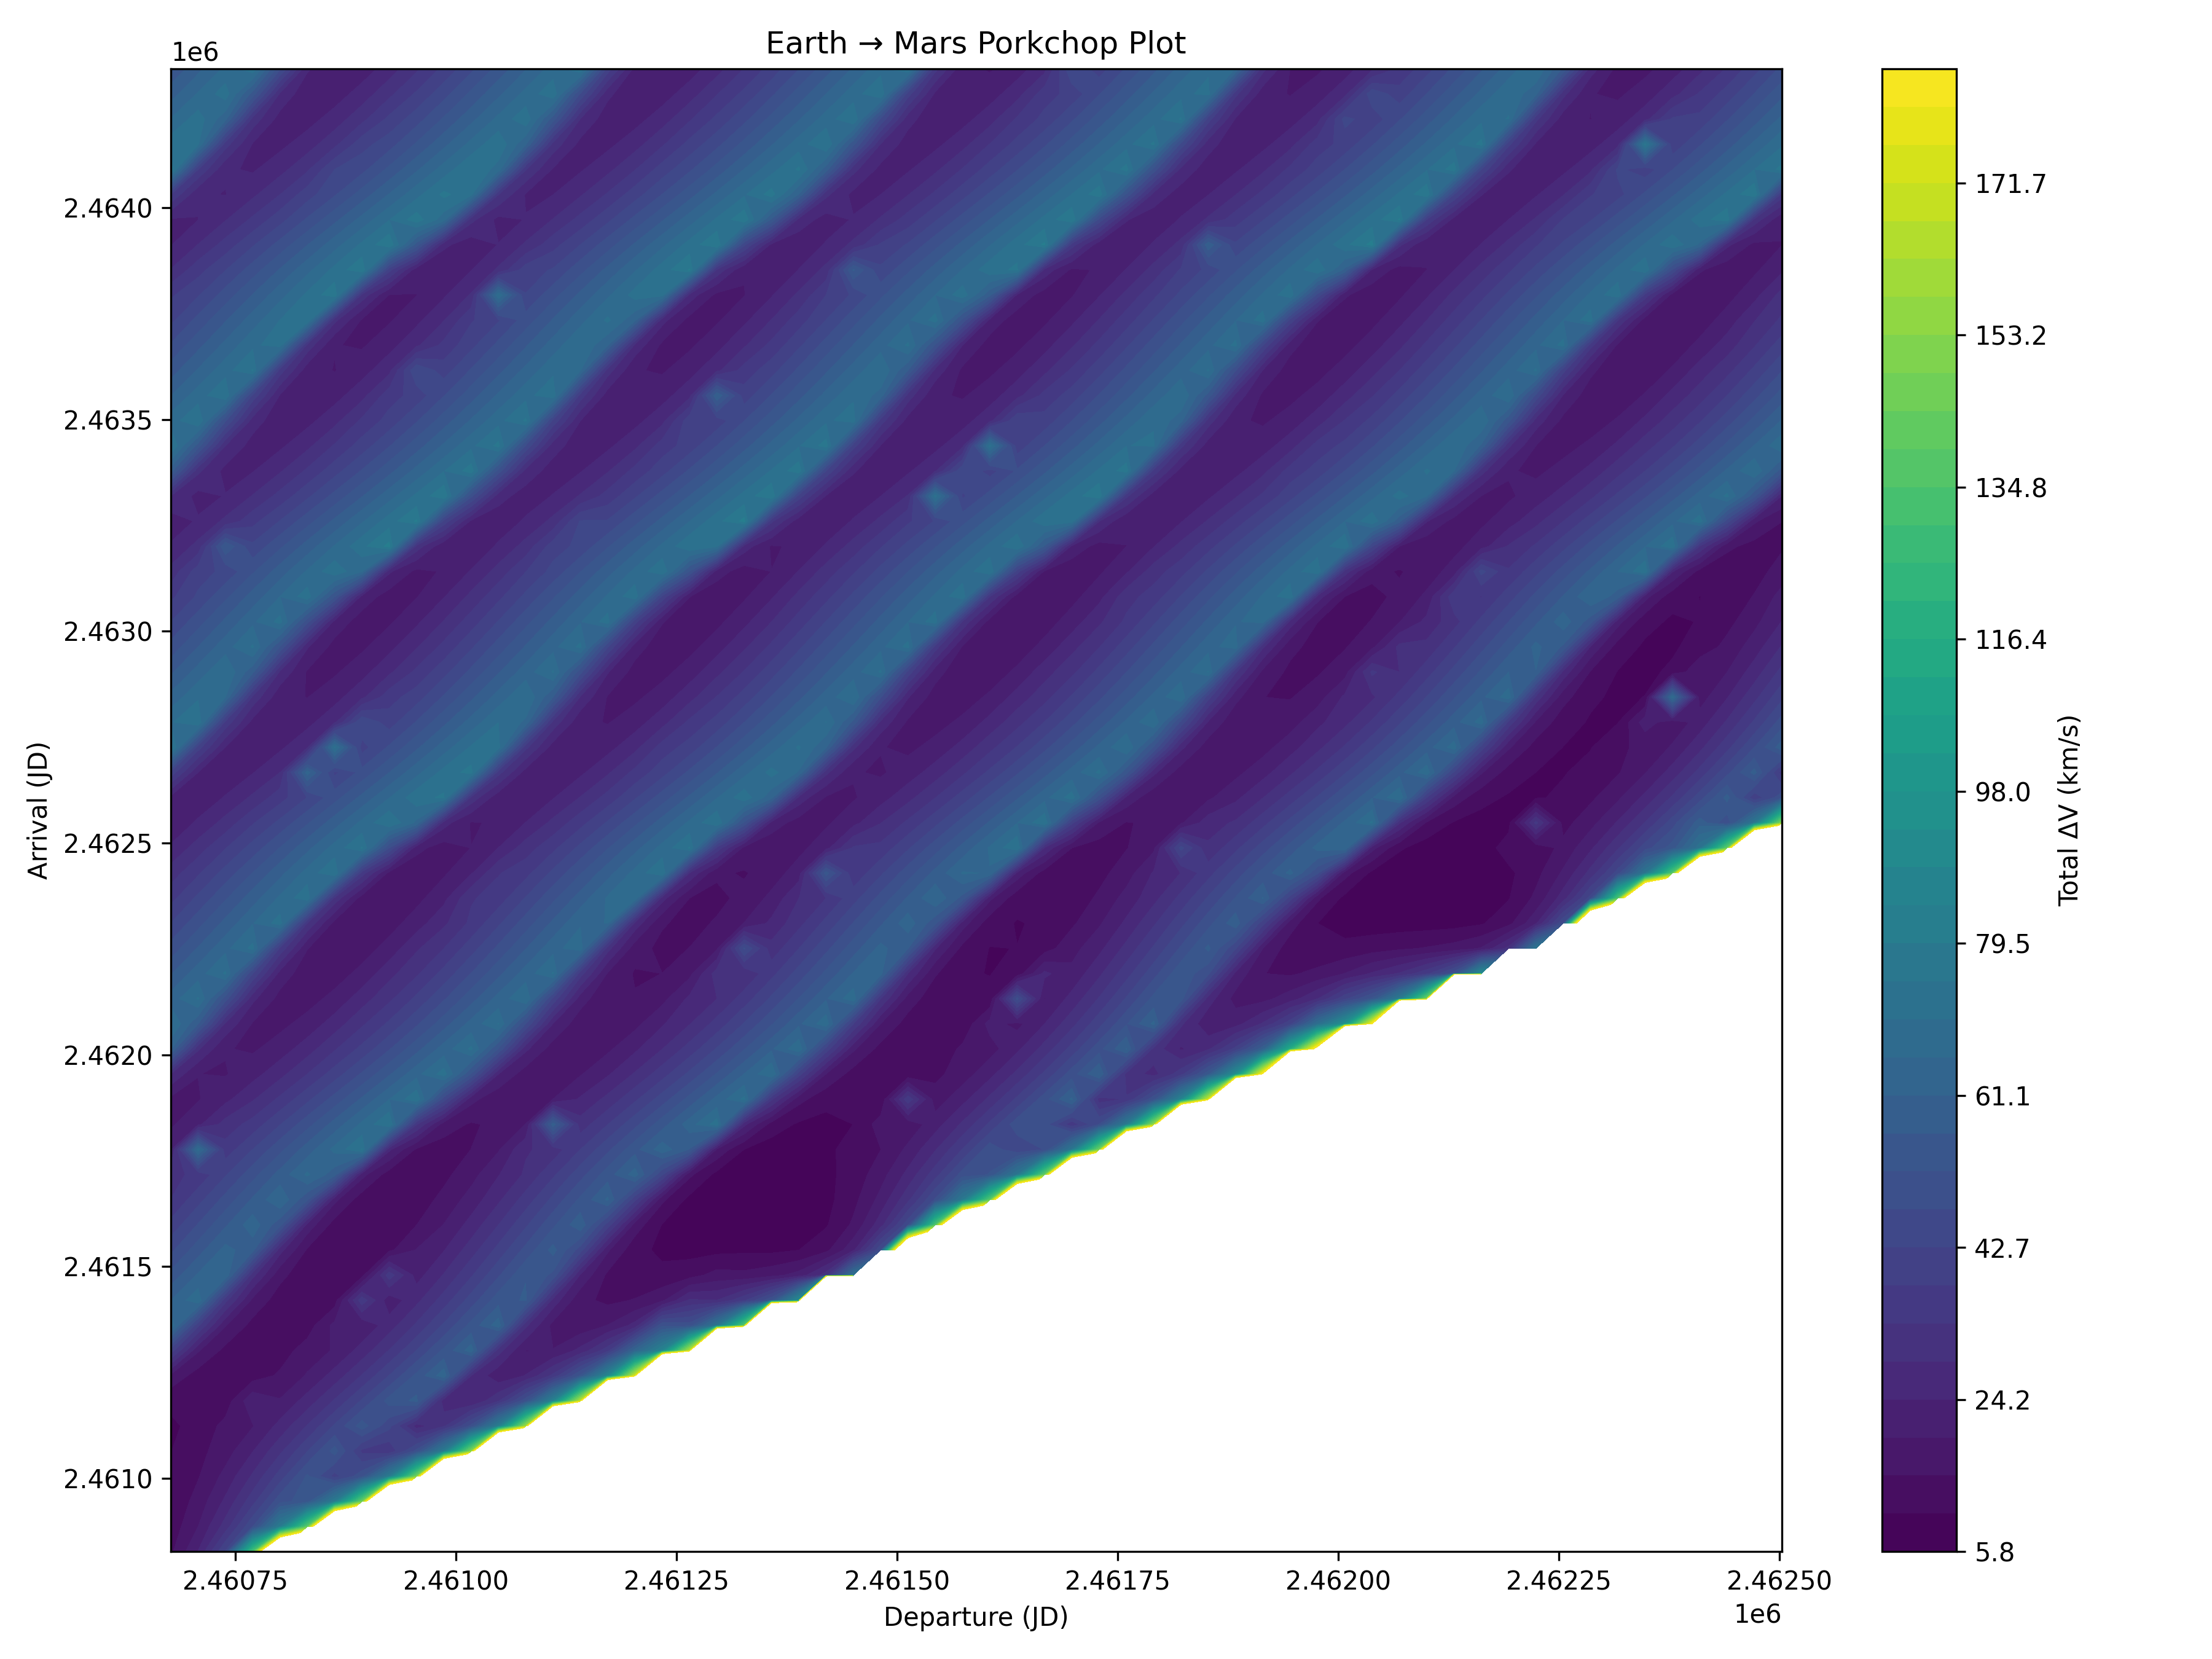
\includegraphics[width=0.42\textwidth]{porkchop.png}
		\caption{Synthetic Earth--Mars pork-chop surface showing $\Delta V$ contours (color) as a function of departure epoch and TOF. Blue regions indicate low-energy transfer windows.}
		\label{fig:dataset}
	\end{figure}
	
	\section{Data Training and Independent Testing Method}
	The surrogate model will be trained on the primary dataset and independently tested on unseen launch configurations. Performance will be evaluated using quantitative error metrics and qualitative visual comparisons to the baseline pork-chop surface. This structure is analogous to the workflows in Ruff \textit{et al.}~\cite{ruff2023surrogate}, where surrogates are validated on trajectory-planning tasks not seen during training.
	
	\section{Validation Metrics}
	\begin{itemize}
		\item Mean Absolute Error (MAE) [km/s]
		\item Root Mean Squared Error (RMSE)
		\item Coefficient of Determination ($R^2$)
		\item Relative evaluation time compared to the numerical solver
	\end{itemize}
	These metrics are standard in surrogate-based optimization studies and help compare accuracy and efficiency trade-offs~\cite{ruff2023surrogate}.
	
	\section{Expected Flow and Connections}
	The project demonstrates a clear and structured flow:
	\begin{enumerate}
		\item Synthetic pork-chop dataset generation provides labeled examples.
		\item The surrogate model approximates the relationship between launch parameters and $\Delta V$, supporting fast trade-space exploration.
		\item Validation metrics measure both predictive accuracy and computational efficiency, echoing evaluation strategies from surrogate and RL-based trajectory studies~\cite{zavoli2021reinforcement,federici2024robust,ruff2023surrogate}.
		\item Results and methodology are documented through six Google Colab tutorials covering dataset setup, model description, optimization, testing, refinement, and full workflow execution.
	\end{enumerate}
	
	\section{Conclusion}
	This proposal outlines a data-driven approach to approximating Earth--Mars pork-chop surfaces using a surrogate model trained on numerically generated transfer data. By drawing inspiration from reinforcement learning approaches to robust trajectory design~\cite{zavoli2021reinforcement,federici2024robust} and from surrogate neural networks for simulation-based optimization~\cite{ruff2023surrogate}, the project aims to demonstrate how even a relatively small-scale surrogate can provide meaningful runtime reductions and intuitive visualizations for early mission design.
	
	\begin{thebibliography}{00}
		
		\bibitem{zavoli2021reinforcement}
		A.~Zavoli and L.~Federici, ``Reinforcement learning for robust trajectory design of interplanetary missions,'' \textit{Journal of Guidance, Control, and Dynamics}, vol.~44, no.~8, pp.~1447--1459, 2021.
		
		\bibitem{ruff2023surrogate}
		E.~Ruff, R.~Russell, M.~Stoeckle, P.~Miotto, and J.~P.~How, ``Surrogate neural networks for efficient simulation-based trajectory planning optimization,'' arXiv preprint arXiv:2303.17468, 2023.
		
		\bibitem{federici2024robust}
		L.~Federici \textit{et al.}, ``Robust interplanetary trajectory design under multiple uncertainties via meta-reinforcement learning,'' \textit{Acta Astronautica}, vol.~214, pp.~147--158, 2024.
		
	\end{thebibliography}
	
\end{document}
